\section{An Accurate Performance Model}
This section introduces a new performance model constructed to accurately predict the execution time of the MapReduce job in the Hadoop cluster.

To construct an accurate performance model, there are some effective methods and principles as follows:
\begin{itemize}
\item To accurately predict the execution time of the MapReduce job, this performance model should be able to forecast each execution phase's cost of the job accurately.
\item The output of each execution phase is the input of the next execution phase, hence this model also needs to forecast the volume of each phase's output beside the execution cost.
\item The execution time of the map and reduce task is not the sum of each phase's cost, due to the presence of parallel that multiple phases execute simultaneously. In order to construct an accurate model, it's necessary to confirm whether the parallel exists between multiple phases, and to predict the overlap time between these phases executed in parallel.
\end{itemize}

The execution of a MapReduce job consists of the map and reduce tasks, hence the construction of the performance model is divide two sections as follows.

\subsection{The Cost Model For Map Task}
The execution of the map task, which is described in the section 2, consists of the following phases: read, map, spill and merge. The key of our work is to predict the actual cost of map and spill.

\noindent\textbf{Map and Spill. }The user-defined map function is executed by the main thread to process the input data, and the spill of the buffer data is performed by the spill thread to sort, combine and write the buffer data sequentially.

\noindent\textbf{(i) Execution Procedure}
\begin{figure}[htbp]
\centering
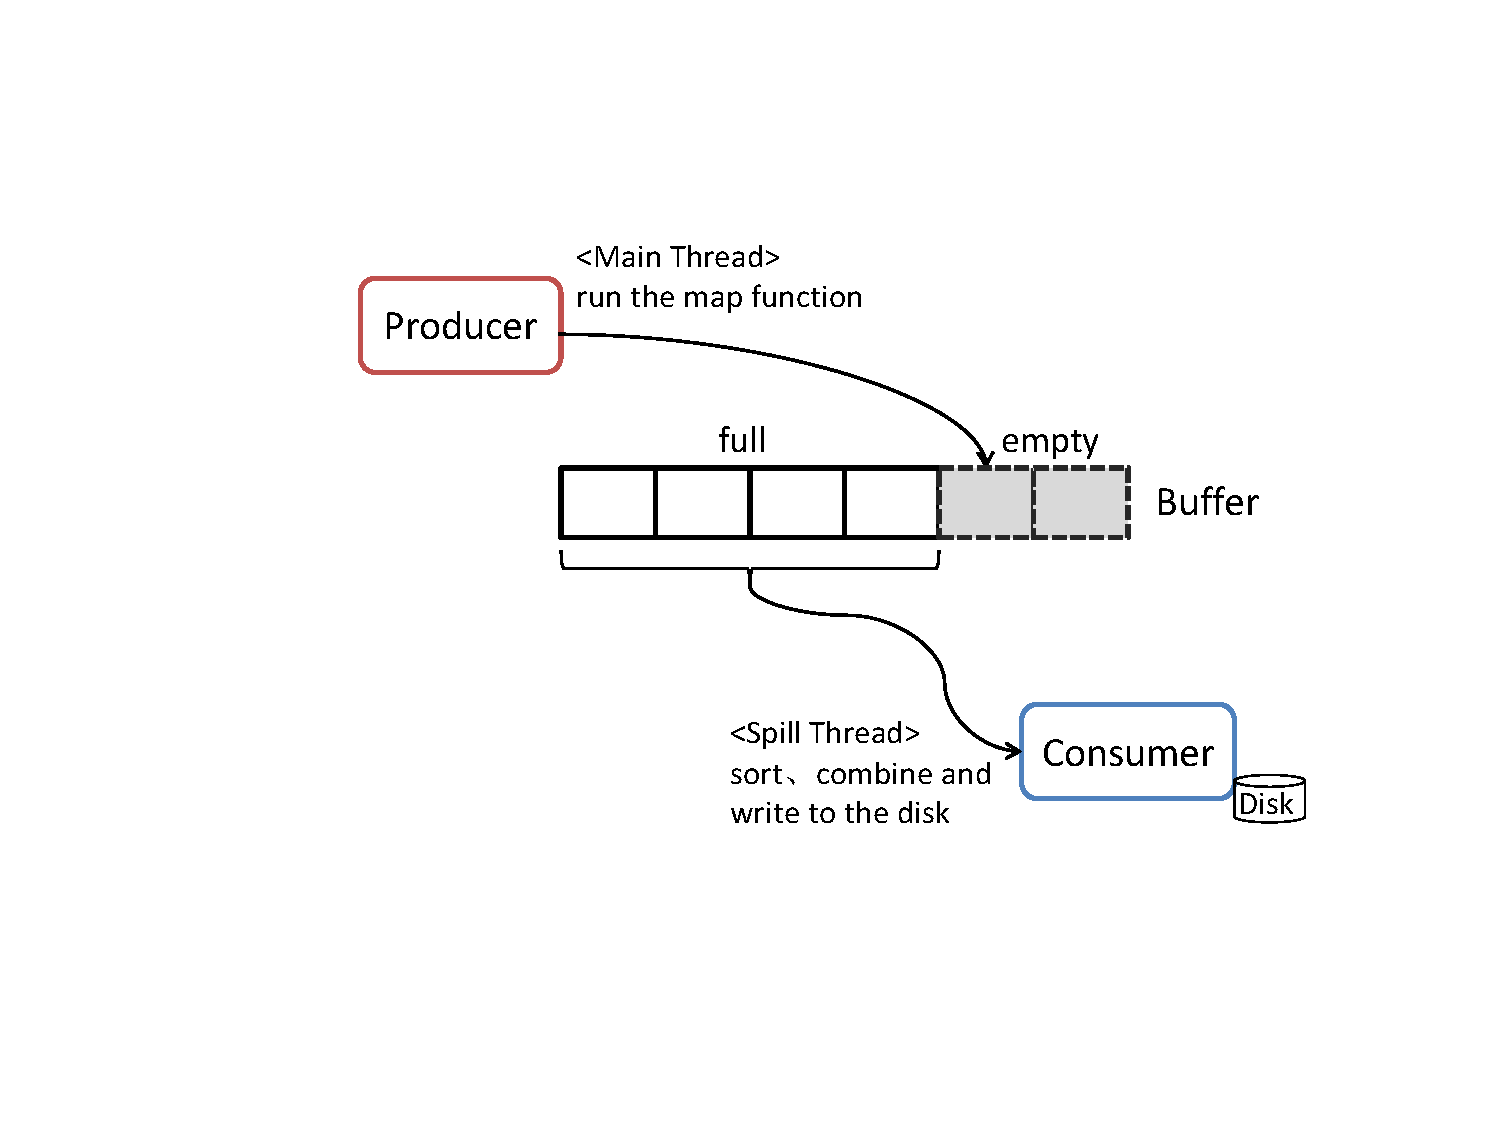
\includegraphics[height=4.5cm, width=8cm]{mapandspill}
\caption{The Interaction between Map and Spill}
\end{figure}

As shown in figure 3, when the main thread executes the map function, the output of the map function is written into the memory buffer. The spill thread starts to spill the outputs cached in the buffer to the disk file when the used space of the buffer reaches the threshold determined by the related configuration parameter. The main thread continues to execute the map function, when the spill thread spills the data into the disk file. The main thread starts to sleep when the buffer is full and stop sleeping after the data in the buffer is written to disk file.

\noindent\textbf{(ii) The Analysis of Key Effect Factors}
\begin{itemize}
\item  \textbf{The cost of map function's execution every time} $m_{cs}$, and \textbf{the number of map function's execution} $mn_d$. The factor $m_{cs}$ is determined by not only the complexity of the user-defined map function but also the execution environment which consists of the resource consumed by map task and the number of executing threads in the map task.
\item  \textbf{The size of memory buffer} $mb_p$, and \textbf{the threshold at which the spill is triggered} $st_p$. These two factors determine when to spill.
\end{itemize}

The total execution time of map and spill is not their linear additivity, due to the parallel execution between map and spill. To predict the total cost of these two phases, we need to estimate not only the individual cost of map and spill, but also their overlap time during which these two phases execute simultaneously. The cost of map is determined by the $m_{cs}$ and $mn_d$, and the cost of spill is determined by the cost of one spill $os_c$ and the number of spill affected by the $mb_p$ and $st_p$. If the $mb_p$ and $st_p$ increase, the $os_c$ increases but the number of spill decreases, therefore it's uncertain whether the cost of spill increases or not. Their overlap time is determined by the $os_c$ and the cost of map when spilling $mws_c$ which is also affected by the $mb_p$ and $st_p$. when the $mb_p$ is fixed, if the $st_p$ increases, the $os_c$ increases but the $mws_c$ might decreases or increases(it's determined by whether the main thread is sleep or not), therefore it's also uncertain whether the overlap time increases or not. In summary, it's challenging to estimate the total execution time of map and spill which is nonlinearly affected by these key factors. We construct the following model to predict the total execution time of map and spill.


\noindent\textbf{(iii) The Construction of Model}

We propose a model to predict the total execution time of map and spill as follows. We need to predict the dataflow of these two phases before estimating the cost.

\emph{DATAFlOW}: The dataflow of these two phases consists of the input and output of each phase. We estimate the output of each phase through the output of last phase and the dataflow statistics captured by the LTrace, for example, the output of map is estimated as follows.
\begin{small}
$$mor_d=mn_d\times\frac{\sum_{i=1}^nmrs_{ds}^i}{n}$$
\end{small}
\emph{where the $mor_d$ is the total number of output records generated by the map function, the $mn_d$ is the number of input records to be processed by the map function, and the $mrs_{ds}^i$ is the records selectivity of the map function performed on the $i$th machine. }
\begin{small}
$$mob_d=mib_d\times\frac{\sum_{i=1}^nmbs_{ds}^i}{n}$$
\end{small}
\emph{where the $mob_d$ is the total size of output bytes generated by the map function, the $mib_d$ is the size of input bytes to be processed by the map function, and the $mbs_{ds}^i$ is the sizes selectivity of the map function performed on the $i$th machine. }
\begin{small}
$$morw_d=\frac{mob_d}{mor_d}$$
\end{small}
\emph{where the $morw_d$ is the average size of each output record generated by the map function.}

Similarly, we estimate the input and output of the spill which consist of the number of records per spill $rps_d$, the number of output records per spill $sor_d$, the size of output bytes per spill $sob_d$, and the number of spills $ns_d$.

\emph{COST}: To predict the total execution time of these two phases, we have to estimate the costs of these two phases and their overlap time as follows.
\begin{small}
\begin{equation}
\begin{split}
mas_c=s_c+ls_c+m_c-otms_c
\end{split}
\end{equation}
\end{small}
\emph{where the $mas_c$ is the total execution time of these two phases, the $s_c$ is the cost of all the spills except the last, the $ls_c$ is the cost of last spill executed by the main thread, the $m_c$ is the cost of the map, and the $otms_c$ is the overlap time between these two phases.}

To predict the total execution time $mas_c$, it's essential to accurately predict the $s_c$, $ls_c$, $m_c$ and the $otms_c$.

The $cSpillCost$ is estimated as follows.
\begin{small}
\begin{equation}
\begin{split}
s_c=ns_d\times os_c
\end{split}
\end{equation}
\end{small}
\emph{where the $ns_d$ is the number of spills executed by the spill thread, and the execution cost per spill $os_c$ which is estimated as follows.}
\begin{small}
\begin{equation}
\begin{split}
os_c=rps_d\times\frac{\sum_{i=1}^ns_{cs}^i}{n}+rps_d\times\frac{\sum_{i=1}^nc_{cs}^i}{n}+sob_d\times \frac{\sum_{i=1}^nw_{cs}^i}{n}\nonumber
\end{split}
\end{equation}
\end{small}
\emph{where the $rps_d$, $rps_d$ and $sob_d$ are estimated by the means introduced above, and the $s_{cs}^i$, $c_{cs}^i$ and the $w_{cs}^i$ are respectively the cost statistics about sorting, combining and writing}

The cost of last spill $ls_c$ is estimated as follows.
\begin{small}
\begin{equation}
\begin{split}
ls_c=(mor_d-ns_d\times rps_d)\times \frac{\sum_{i=1}^ns_{cs}^i}{n}+(mor_d\\
-ns_d\times rps_d)\times \frac{\sum_{i=1}^nc_{cs}^i}{n}+morw_d\times  (mor_d\\
-ns_d\times rps_d)\times \frac{\sum_{i=1}^ncb_{ds}^i}{n}\times \frac{\sum_{i=1}^nw_{cs}^i}{n}
\end{split}
\end{equation}
\end{small}
\emph{where the $ls_c$ is composed of the costs of sorting, combining and writing the buffer data into a new disk file, and the $cb_{ds}^i$ is the data statistics about combining. }

Through the above analysis of the key effect factors, the cost of map function's execution every time is effected by the number of executing threads in the map task. The main thread may execute the map function when the spill thread is spilling the data cached in the buffer into a new file, and the execution speed of the map function is slower due to the simultaneous execution of the spill thread. Therefore, the execution cost of map is divided into two parts as follows.
\begin{small}
\begin{equation}
\begin{split}
m_c=mws_c+mns_c
\end{split}
\end{equation}
\end{small}
\emph{where the $m_c$ is the total execution time of map, the $mws$ is the execution time of map when the spill thread is running and the $mns_c$ is the execution time of map when the spill thread is stopping.}

The spill thread spills the data cached in the buffer in parallel with the main thread which executes the map function, due to the remaining space of the buffer. The main thread starts to sleep when the buffer is full, and the main thread restarts to execute the map function when the spill is completed. Therefore, the estimation of the $mws_c$ and $mns_c$ is complicated, which is closely associated with the remaining space of the buffer.

We assume that there are not enough remaining space in the buffer to hold the output of the map function when the spill thread is executing, and the execution time of the main thread when the spill thread is working is less than the cost of one spill due to the sleep of the main thread. This assumption is judged as follows.
\begin{small}
\begin{equation}
\begin{split}
isMainThrSleep=mwos_c<os_c \nonumber
\end{split}
\end{equation}
\end{small}
\emph{where the $mwos_c$ is the cost of the map when the spill thread is executing, and it is estimated as follows,}
\begin{small}
\begin{equation}
\begin{split}
mwos_c=\frac{mb_p\times (1-st_p)}{(morw_d+16)} \times\frac{\sum_{i=1}^nmws_{cs}^i}{\sum_{i=1}^nmrs_{ds}^i} \nonumber
\end{split}
\end{equation}
\end{small}
\emph{where the $mws_{cs}^i$ is the cost of map function's execution every time when the spill thread is running on the $i$th machine, and it is captured by the LTrace.}

When the above assumption is tenable, the main thread starts to sleep when the buffer is full, and the $mws_c$ and $mns_c$ are estimated as follows.
\begin{small}
\begin{equation}
\begin{split}
mws_c=mwos_c\times (ns_d-1)+Min(\frac{mb_p\times (1-st_p)}{(morw_d+16)} ,mor_d\\
-rps_d\times ns_d)\times \frac{\sum_{i=1}^nmws_{cs}^i}{\sum_{i=1}^nmrs_{ds}^i} \nonumber
\end{split} 
\end{equation}
\end{small}
\begin{small}
\begin{equation}
\begin{split}
mns_c=(mor_d-(ns_d-1 )\times\frac{mb_p\times (1-st_p)}{(morw_d+16)}-Min(mor_d\\
 - rps_d\times ns_d, \frac{mb_p}{(morw_d+16)} 
\times (1-st_p)))\times \frac{\sum_{i=1}^nm_{cs}^i}{\sum_{i=1}^nmrs_{ds}^i} \nonumber
\end{split}
\end{equation}
\end{small}
\emph{where the $m_{cs}^i$ is the cost of map function's execution every time when the spill thread is not running on the $i$th machine, and it is captured by the LTrace.}

When the above assumption is not tenable, the main thread does not sleep due to the enough space of the buffer. The $mws_c$ and $mns_c$ are estimated as follows.
\begin{small}
\begin{equation}
\begin{split}
mws_c=nmws_d \times\frac{\sum_{i=1}^nmws_{cs}^i}{n} \nonumber
\end{split}
\end{equation}
\end{small}
\begin{small}	
\begin{equation}
\begin{split}
mns_c=nmns_d\times \frac{\sum_{i=1}^n m_{cs}^i}{n} \nonumber
\end{split}
\end{equation}
\end{small}
\emph{where the $nmws_d$ is the number of map function's execution when the spill thread is running, and the $nmns_d$ is the number of map function's execution when the spill thread is sleeping, and they are estimated as follows.}
\begin{small}
\begin{equation}
\begin{split}
nmws_d=\frac{os_c\times n}{\sum_{i=1}^n mws_{cs}^i} \times 
(ns_d-1)+Min( \frac{os_c\times n}{\sum_{i=1}^n mws_{cs}^i} 
, \\
\frac{(mor_d-ns_d\times rps_d)\times n}{\sum_{i=1}^nmrs_{ds}^i})  \nonumber
\end{split}
\end{equation}
\end{small}
\begin{small}
\begin{equation}
\begin{split}
nmns_d=mn_d-nmws_d \nonumber
\end{split}
\end{equation}
\end{small}
At last, the $otms_c$ is estimated as follows.
\begin{small}
\begin{equation}
\begin{split}
otms_c=mws_c
\end{split}
\end{equation}
\end{small}
\subsection{The Cost Model For Reduce Task}
The execution of the map task, which is described in the section 2, consists of the following phases: shuffle, merge, reduce and write. The key of our work is to predict the effective cost of shuffle.

\noindent\textbf{Shuffle.} The reduce task reads the corresponding outputs of all the map tasks from the remote machines in the cluster.

\noindent\textbf{(i) Execution Procedure}
\begin{figure}[htbp]
\centering
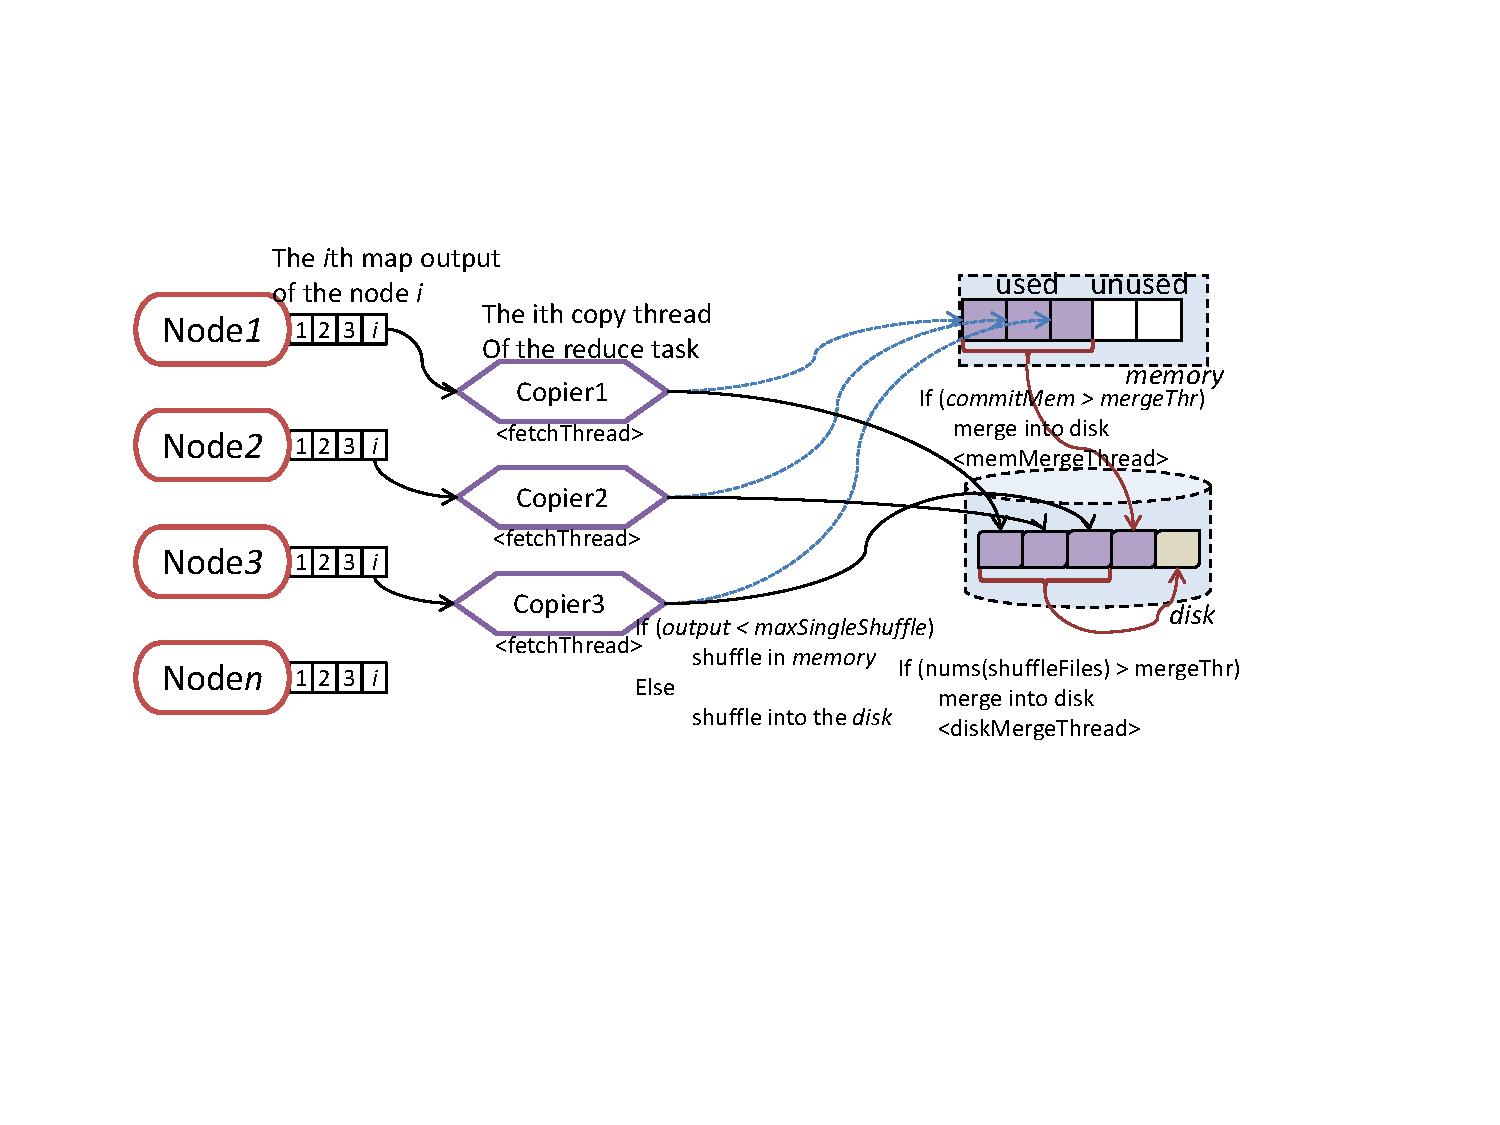
\includegraphics[height=4.5cm, width=9cm]{shuffle}
\caption{The Execution Procedure of Shuffle}
\end{figure}

As shown in figure 4, multiple copy threads of the reduce task are started to simultaneously fetch the corresponding outputs of map tasks from the various machines When there are multiple outputs generated by different map tasks on a machine, only one of these copy threads sequentially fetches these outputs from the target machine.

When the copy thread starts to fetch the output of the completed map task, the output can be written to the memory buffer or a new disk file, which
is determined by the way as shown in figure 4. A merge thread is started, when the used space of the memory buffer or the number of disk files reach the threshold.

\noindent\textbf{(ii) The Analysis of Key Effect Factors}
\begin{itemize}
\item \textbf{The number of the effective copy threads} $nc_p$, the $nc_p$ is the actual number of copy threads which simultaneously fetch the outputs of map tasks from $nc_p$ machines.
\item \textbf{The output of the map task} $mo_d$, and \textbf{the max single shuffle limit} $mssl_p$. These two factors determine whether the map task's output is fetched into the buffer or disk.
\item \textbf{The threshold at which the memory merge is triggered} $mt_p$, and \textbf{the number of disk files at which the disk merge is triggered} $sf_p$. These two factors affect when the merge thread merge the buffer data or the disk files into a new file.
\end{itemize}

\noindent\textbf{(iii) The Construction of Model}

We propose the simulation approach to predict the whole shuffle time of the reduce task. 

\noindent\rule{3.5in}{0.6mm}
\textbf{Algorithm 1} The simulation of shuffling into the buffer
\rule{3.5in}{0.3mm}
\begin{algorithmic}[1]
\Require $mapOutputs$, $numCopies$
\Ensure $cShuffleTime$
\Function{CShMCost}{$mapOutputs, numCopies$}
\State $T_c \gets 0,  T_m \gets 0, T_d \gets 0$
\State $haveShu\gets 0, isM \gets 0, isF \gets 0 $
\State $Outs_m \gets null, Outs_d \gets null $
\State $numOuts_{mtod} \gets 0, copyDests \gets null $
\State $indexDest \gets 0$
\For{$i=0 \to numCopies-1$}
\If{$i<length[mapOutputs]$}
\State $copyDests[i] \gets mapOutputs[i]$
\State $indexDest \gets indexDest + 1$
\Else
\State $copyDests[i] \gets null$
\EndIf
\EndFor
\While{!\Call{IsNull}{$mapOutputs$}}
\For{$t=0 \to numCopies - 1$}
\State $out \gets copyDest[t] $
\If{$out \neq null$ \textbf{and} $T_c >= T_s[out]$}
\State $nums[out] \gets nums[out] - 1$
\State $Outs_m \gets Outs_m + out$
\State $haveShu \gets 1$
\If{\Call{IsMerge}{$MapOuts_m$}}
\State $isM \gets 1$
\State $numOuts_{mtod} \gets size[Outs_m]$
\EndIf
\If{$nums[out] == 0 $}
\State \Call{UpdateCopyDest}{$indexDest,$
        $mapOutputs$}
\EndIf
\If{\Call{IsFull}{$MapOuts_m$}}
\State $isF \gets 1$
\State exit
\EndIf

\EndIf
\EndFor
\If{$havaShu == 1$}
\State $T_c \gets T_c + \Call{ShuCost}{mapOutputs[0]}$
\State $haveShu \gets 0$
\If{$isM == 1$}
\State $T_m \gets \Call{Max}{T_c, T_m}$
\State $T_m \gets T_m + \Call{MemMerge}{$
$MapOuts_m, numOuts_{mtod}, Outs_d}$

\If{$\Call{IsDiskMerge}{Outs_d}$}
\State $T_d \gets \Call{Max}{T_d, T_m}$
\State $T_d \gets \Call{DiskMerge}{Outs_d} + T_d$
\EndIf
\State $isM \gets 0$
\EndIf

\If{$isF == 1$}
\State $\Call{RemoveMemOuts}{Outs_m, $
$numOuts_{mtod}}$
\State $T_c = \Call{Max}{T_c, T_m}$
 \State $isF \gets 0$
\EndIf

\Else
\State $T_{new} \gets \Call{LastedClock}{mapOutputs}$
\State $T_c \gets \Call{Max}{T_c, T_{new}}$
\EndIf

\EndWhile
\State $cShuffleTime \gets \Call{Max}{T_c, T_m, T_d}$
\EndFunction
\end{algorithmic}
\noindent\rule{3.5in}{0.6mm}

In the algorithm 1, the $mapOutputs$ is the set of the map task's outputs on all the machines, each element of this set records the number and the finish time of map tasks simultaneously executing on the one machine. The $T_c$, $T_m$ and $T_d$ respectively are the clock of copy thread, memory merge thread and the disk merge thread, and these clocks record the start or end time of the related trigger event, for example, the $T_m$ records the start and end time of the memory merge executed by the memory merge thread. When a event is trigger by one thread, the start time of the event is updated to be the current clock of that certain thread, and the end time of the event is the sum of this event's cost and the start time. For example, if the buffer data size reach the memory merge threshold after one copy thread fetches the data into the buffer, the memory merge event is trigger, the start time of this memory merge $T_m$ is updated to be the copy thread's clock $T_c$, and then the $T_m$ increases by the cost of this merge thread, which presents the end time of this event. The value of $isM$ indicates whether it's time to start to memory merge thread to merge the buffer data into a new file, and the $isF$ indicates whether the buffer is full. The $Outs_m$ and $Outs_d$ are the outputs of map tasks stored in the memory and disk respectively. The value of $haveShu$ indicates that whether there are map tasks' outputs to be fetched at the moment, if the $haveShu$ is 0, then the $T_c$ needs to be updated as the latest finish time of all the remaining map tasks. The $cShuffleTime$, the cost of shuffle, is the maximum of $T_c$, $T_m$, $T_d$. It is worth to note that our algorithm can predict the effective shuffle time of the reduce task, when there are multiple waves of map tasks and reduce tasks simultaneously running on this cluster.

Similar to the algorithm 1, we can use the similar method to calculate the cost of the shuffle, when the map tasks' outputs are written into the disk.  The $T_c$ and $T_d$ respectively are the clock of copy thread and disk merge thread, and the maximum of the $T_c$ and $T_d$ is the shuffle cost $cShuffleTime$.

